\documentclass[10pt]{beamer}


\usetheme[nosectionslide,everytitleformat=regular]{m}

% camel case
% \renewcommand{\mthemetitleformat}{}

\definecolor{mDarkRed}{HTML}{8F0129}
\definecolor{mGreen}{HTML}{0E8740}

\definecolor{BrickRed}{HTML}{B6321C}
\definecolor{DarkOrchid}{HTML}{A4538A}
\definecolor{ForestGreen}{HTML}{009B55}
\definecolor{Goldenrod}{HTML}{897E4D}

\setbeamercolor{alerted text}{fg=mGreen}
\setbeamertemplate{bibliography item}[text]

\setbeamertemplate{footnote}{\hangpara{2em}{1}\makebox[2em][l]{\insertfootnotemark}\footnotesize\insertfootnotetext\par}


\usepackage[scale=2]{ccicons}

\usepackage{cmap}           % Mapeamento de caracteres especiais no PDF
\usepackage{lmodern}        % Usa fonte Latin Modern
\usepackage[T1]{fontenc}    % Seleção de codificação de fonte
\usepackage[utf8]{inputenc} % Codificação do arquivo (conversão automática dos acentos)
\usepackage[brazil]{babel}  % Idioma para hifenização e tradução de vários elementos
\usepackage{makeidx}        % Criação de índice
\usepackage{hyperref}       % Formatação do índice
\usepackage{lastpage}       % Usado pela Ficha catalográfica
\usepackage{indentfirst}    % Indenta o primeiro parágrafo de cada seção
\usepackage{graphicx}       % Inclusão de gráficos
\usepackage{booktabs}       % Formatação de tabelas
% -------------------------------------------------------------------------------------------------
% Para citações
% \usepackage[brazilian,hyperpageref]{backref} % Páginas com as citações na bibliografia
\usepackage[alf]{abntex2cite} % Citações padrão ABNT (alfanumérico)
% -------------------------------------------------------------------------------------------------
% Pacotes opcionais
\usepackage{nomencl}        % Para criar uma lista de símbolos
\usepackage{acro}           % Para usar acrônimos e abreviaturas
\usepackage{tikz}           % Para fazer figuras, diagramas e gráficos integrados e elegantes
\usepackage{pgfplots}       % Usa o pacote tikz para fazer gráficos muito melhores que os do Excel
\usepackage{pgfplotstable}  % Para gerar tabelas automaticamente a partir de arquivos com dados
\usepackage{filecontents}   % Para colocar o conteúdo de um arquivo dentro de um arquivo tex
\usepackage{todonotes}      % Para criar anotações durante o desenvolvimento do texto
%\usepackage{multirow}       % Permite fazer tabelas com múltiplas linhas
\let\newfloat=\undefined    % Workaround para usar o pacote algorithm
\usepackage{algorithm}      % Para escrever algoritmos
\usepackage{algpseudocode}
\usepackage{pifont}
% \usepackage{clrscode}       % Para escrever algoritmos
% \usepackage{clrscode3e}     % Para escrever algoritmos; mais simples que os pacotes acima
\usepackage{pdfpages}        % Para incluir a folha de aprovação assinada em PDF
\usepackage{amsmath}
\usepackage{amsfonts}
\usepackage{mathtools}
\usepackage{subcaption}
\newcolumntype{P}[1]{>{\centering\arraybackslash}m{#1}} 

\usepackage{tablefootnote}
\usepackage{adjustbox}
\usepackage{changepage}
\usepackage{color}

% \usepgfplotslibrary{external} 
% \tikzexternalize


\captionsetup{labelformat=empty,labelsep=none}
\def\multiset#1#2{\ensuremath{\left(\kern-.3em\left(\genfrac{}{}{0pt}{}{#1}{#2}\right)\kern-.3em\right)}}

\makeatletter
\newcommand\footnoteref[1]{\protected@xdef\@thefnmark{\ref{#1}}\@footnotemark}
\makeatother

\DeclareMathOperator*{\argmin}{arg\,min}
\DeclareMathOperator*{\argmax}{arg\,max}


\title{Comparativo de Regressão Logística e Redes Neurais para classificação do XOR}
\subtitle{}
\date{03 de outubro de 2015}
\author[Treviso]{Marcos Treviso\\Sharbell Kemel\\}
\institute{Aprendizado de Máquina - Universidade Federal do Pampa}
\titlegraphic{\hfill
\includegraphics[height=1.25cm]{img/unipampa_logo.png}}

\begin{document}

\maketitle


\begin{frame}
  \frametitle{Roteiro}

  \begin{itemize}

    \item Ambiente de Teste

    \item Resultados

    \item Conclusão

  \end{itemize}

\end{frame}



\begin{frame}
  \frametitle{Roteiro}

  \begin{itemize}

    \item Ambiente de Teste

    \item[\color{gray}{$\bullet$}] \textcolor{gray}{Resultados}

    \item[\color{gray}{$\bullet$}] \textcolor{gray}{Conclusão}

  \end{itemize}

\end{frame}



\section{Ambiente de Teste}

\begin{frame}[fragile]
  \frametitle{Ambiente de Teste}

 \begin{itemize}
      \item Dell Inspiron 7348
    \end{itemize}

    \begin{table}[!htb]
    \footnotesize
    \centering
    \begin{tabular}{ll}
      \toprule
      \textbf{Processador} & Intel i7-5500U 2.40GHz - 4 cores  \\
      \textbf{Memória Principal} & 8 GB RAM DDR3 1600 MHz \\
      \textbf{Cache} & L3 Cache 4 MB \\
      \bottomrule
    \end{tabular}
    \end{table}

  \begin{itemize}
    \item Python 3.4.3
    \item Numpy 1.9.2
  \end{itemize}
  
\end{frame}


\begin{frame}[fragile]
  \frametitle{Ambiente de Teste}

  \begin{itemize}
    \item Regressão Logística:
    \begin{itemize}
      \item[-] Número de iterações, tempo de execução e acurácia
      \item[-] Precisão de $10^{-6}$
      \item[-] Sem regularização
      \item[-] Média de 10 execuções
      \item[-] Otmizador: gradiente descendente
    \end{itemize}

    \item[\ ] \ 
  \end{itemize}


  \begin{itemize}
    \item Redes Neurais
    \begin{itemize}
      \item[-] 1 camada oculta com 10 neurônios
      \item[-] Número de iterações, tempo de execução e acurácia
      \item[-] Precisão de $10^{-6}$
      \item[-] Sem regularização
      \item[-] Sem momentum
      \item[-] 10 épocas
      \item[-] Otmizador: gradiente descendente com backpropagation
    \end{itemize}
  \end{itemize}



\end{frame}


\begin{frame}
  \frametitle{Roteiro}

  \begin{itemize}

    \item[\color{gray}{$\bullet$}] \textcolor{gray}{Ambiente de Teste}

    \item Resultados

    \item[\color{gray}{$\bullet$}] \textcolor{gray}{Conclusão}

  \end{itemize}

\end{frame}



\section{Resultados}

\begin{frame}[fragile]
  \frametitle{Resultados - Regressão Logística}


  \begin{itemize}
    \item Com taxa de aprendizagem igual a 3.0

    \item[\ ] \ 

    \item Diferentes graus do polinômio \multiset{n}{k}

    \item[\ ] \ 

    \item Para $k=2$ e $n = 1, \dots, 60$

    \item[\ ] \ 

    \item Então, $ \dfrac{n \times (n+1)}{2} $ features adicionais


  \end{itemize}



\end{frame}


\begin{frame}
 \frametitle{Resultados - Regressão Logística}

 \begin{itemize}
  \item Variar taxa de aprendizado ($\alpha$)
    \begin{itemize}
      \item (0.01, 0.03, 0.1, 0.3, 1.0, 3.0, 6.0, 12.0, 24.0, 48.0)
    \end{itemize}

  \item Variar grau do polinômio (novas features)
  \begin{itemize}
      \item de 1 até 60
    \end{itemize}

  \item Analisar custo: J(W)

  \item Analisar tempo de execução

  \item Analisar número de iterações

  \item Analisar acurácia

 \end{itemize}

\end{frame}


\begin{frame}
 \frametitle{Resultados - Regressão Logística}

 \begin{itemize}
  \item Com grau do polinômio igual a 2
 \end{itemize}

  \begin{adjustwidth}{-3em}{-3em}
  \begin{figure}[htb]
    \begin{center}
        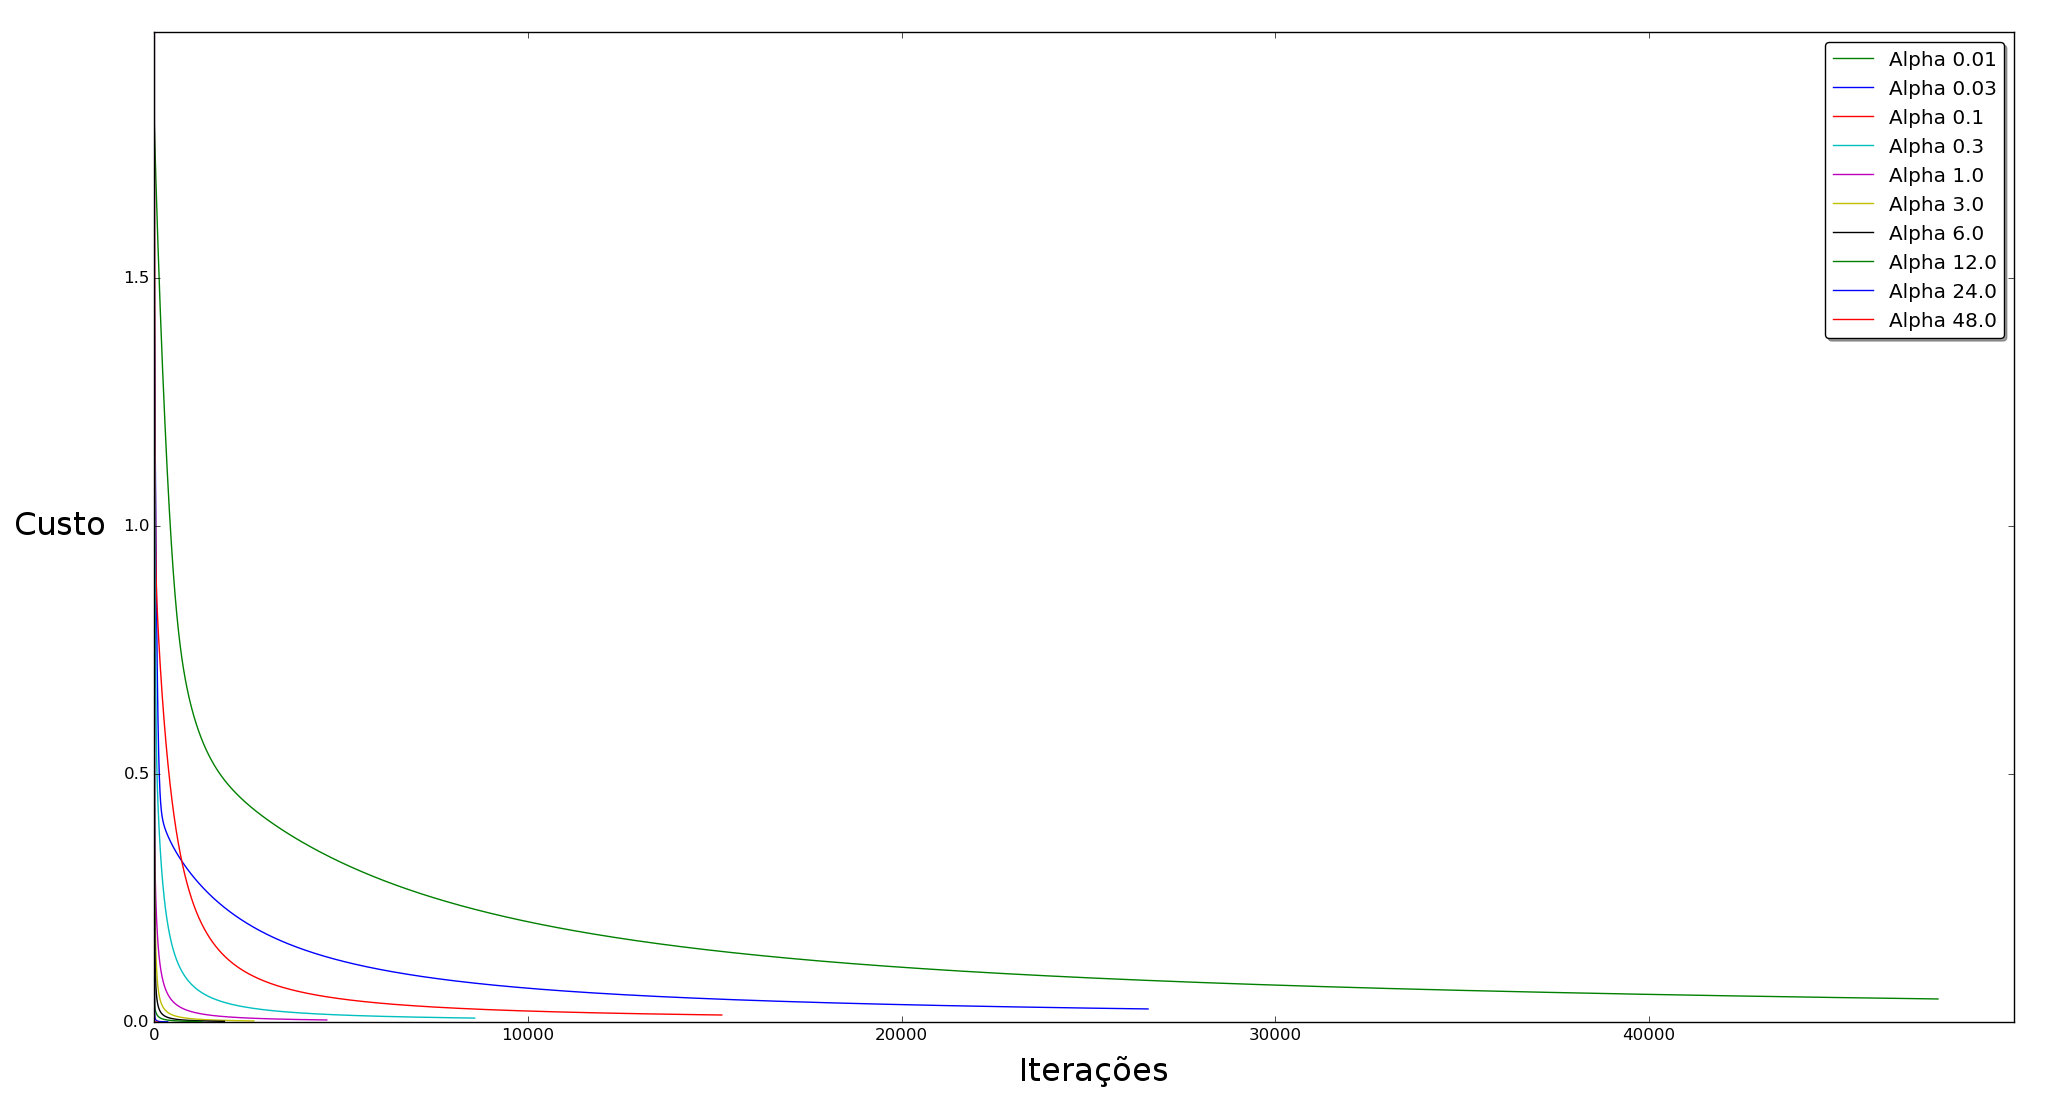
\includegraphics[scale=0.18]{img/alphas_reglog.png}
    \end{center}
    % \caption{Exemplo de classificação gramatical}\label{fig:exemploclassificacao}
  \end{figure}
  \end{adjustwidth}
\end{frame}



\begin{frame}
  \frametitle{Resultados - Regressão Logística}

  \begin{itemize}
  \item Com $\alpha$ igual a 3.0
 \end{itemize}

  \begin{adjustwidth}{-3em}{-3em}

    \begin{figure}[!htb]
    \begin{center}
    \begin{tikzpicture}[scale=1]
      \begin{axis}[
        name=one,
        mlineplot,
        width=1\textwidth,
        height=0.70\textwidth,
        xmode=normal,
        ymode=normal,
        ymin=0,
        ticks=both,
        xlabel=Grau do polinômio,
        ylabel=Tempo de execução (s),
        legend pos=north east,
        legend style={draw=none},
      ]
      \addplot table [x=grau,y=tempo,smooth,header=true,mark=none] {resultados_rl/result_times.txt};
    \end{axis}

    \end{tikzpicture}
  \end{center}
  \end{figure}

  \end{adjustwidth}
\end{frame}



\begin{frame}
  \frametitle{Resultados - Regressão Logística}

  \begin{itemize}
  \item Com $\alpha$ igual a 3.0
 \end{itemize}

  \begin{adjustwidth}{-3em}{-3em}

    \begin{figure}[!htb]
    \begin{center}
    \begin{tikzpicture}[scale=1]
      \begin{axis}[
        name=one,
        mlineplot,
        width=1\textwidth,
        height=0.70\textwidth,
        xmode=normal,
        ymode=normal,
        ymin=0,
        ticks=both,
        xlabel=Grau do polinômio,
        ylabel=Número de iterações,
        legend pos=north east,
        legend style={draw=none},
      ]
      \addplot table [x=grau,y=iters,header=true,mark=none]  {resultados_rl/result_iters.txt};
    \end{axis}

    \end{tikzpicture}
  \end{center}
  \end{figure}

  \end{adjustwidth}
\end{frame}


\begin{frame}
  \frametitle{Resultados - Regressão Logística}

  \begin{itemize}
  \item Com $\alpha$ igual a 3.0
 \end{itemize}

  \begin{adjustwidth}{-3em}{-3em}

    \begin{figure}[!htb]

    \begin{center}
    \begin{tikzpicture}[scale=1]
      \begin{axis}[
        name=one,
        mlineplot,
        width=1\textwidth,
        height=0.70\textwidth,
        xmode=normal,
        ymode=normal,
        ymin=0,
        ticks=both,
        xlabel=Grau do polinômio,
        ylabel=Acurácia (\%),
        legend pos=north east,
        legend style={draw=none},
      ]
      \addplot table [x=grau,y=acc,header=true,mark=none]  {resultados_rl/result_accs.txt};
    \end{axis}

    \end{tikzpicture}
  \end{center}
  \end{figure}

  \end{adjustwidth}
\end{frame}



\begin{frame}
  \frametitle{Resultados - Regressão Logística}

  \begin{itemize}
  \item Com $\alpha$ igual a 3.0
 \end{itemize}

  \begin{adjustwidth}{-3em}{-3em}
  \begin{figure}[htb]
    \begin{center}
        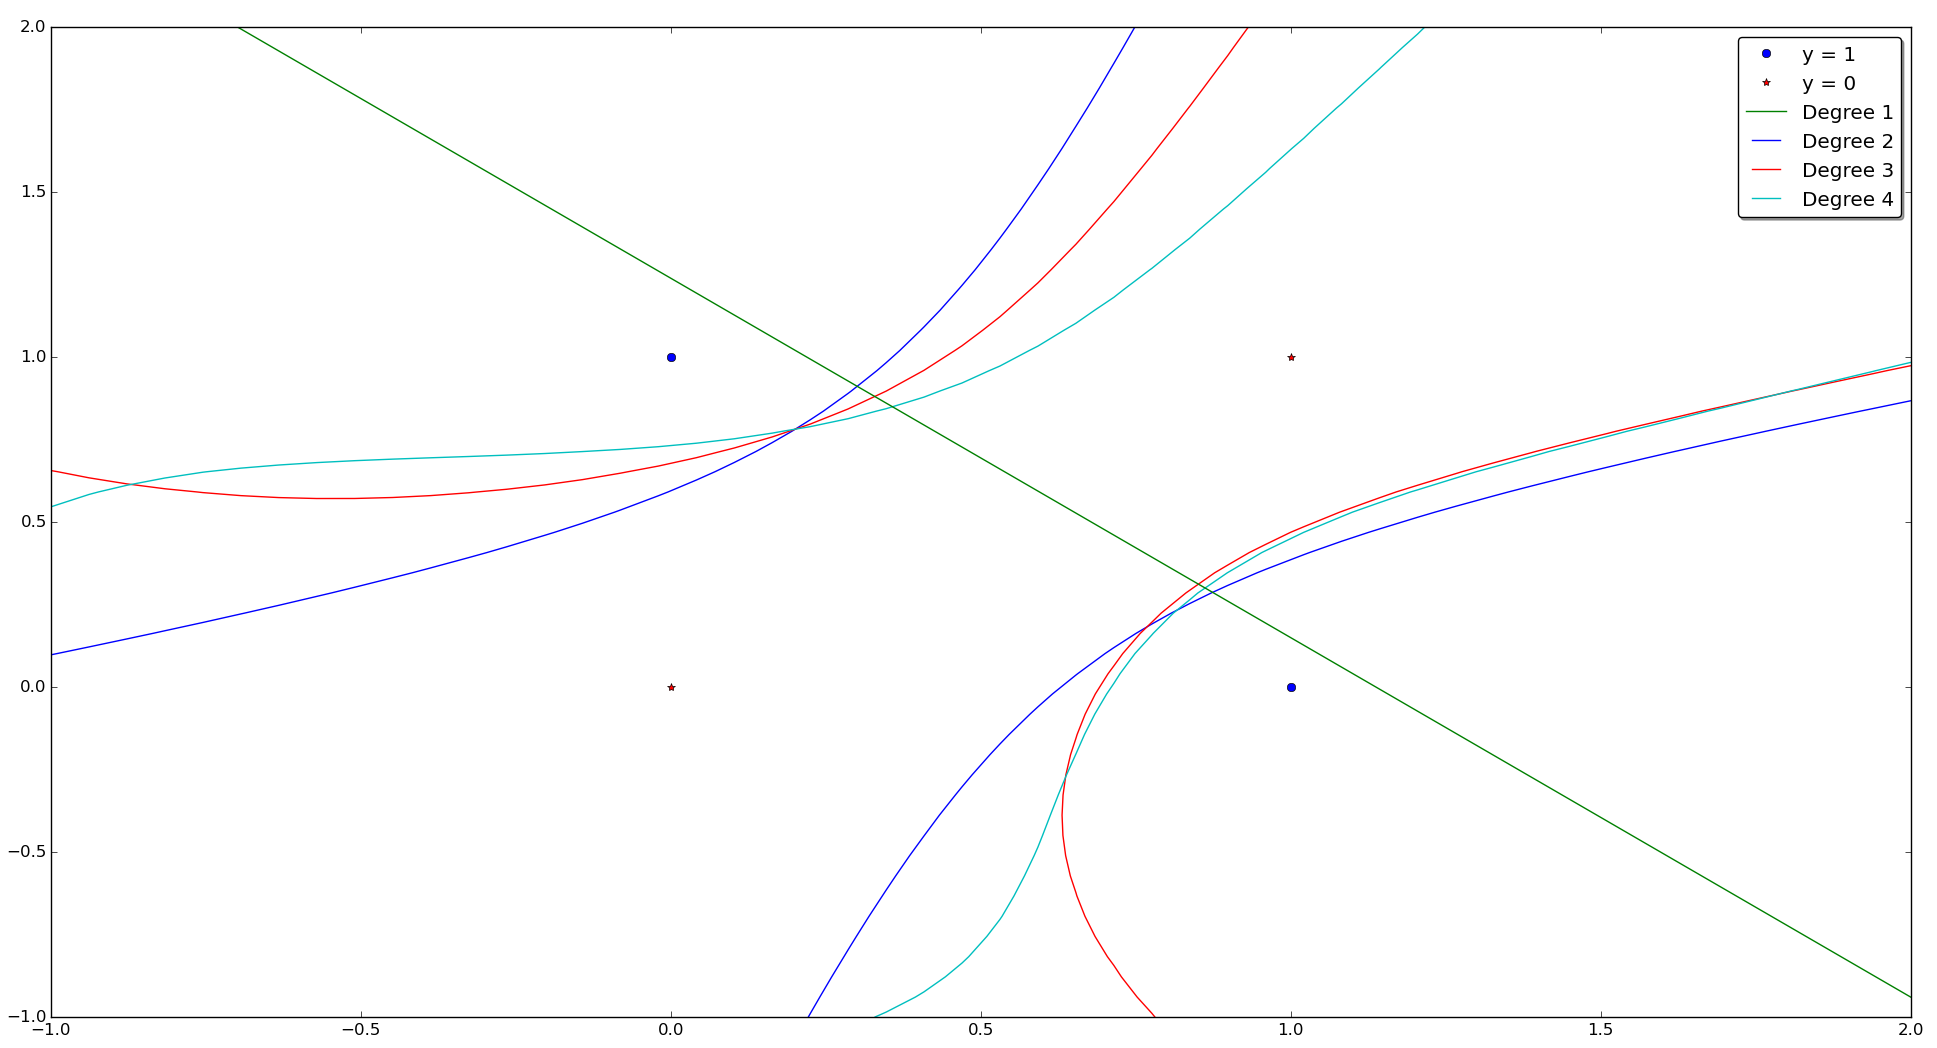
\includegraphics[scale=0.18]{img/decision_boundaries.png}
    \end{center}
    % \caption{Exemplo de classificação gramatical}\label{fig:exemploclassificacao}
  \end{figure}
  \end{adjustwidth}
\end{frame}















\begin{frame}
 \frametitle{Resultados - Redes Neurais}

 \begin{itemize}
  \item Variar taxa de aprendizado ($\alpha$)
    \begin{itemize}
      \item (0.01, 0.03, 0.1, 0.3, 1.0, 3.0, 6.0, 12.0, 24.0, 48.0)
    \end{itemize}

  \item Variar número de unidades ocultas
  \begin{itemize}
      \item de 1 até 6
    \end{itemize}

  \item Analisar custo: J(W)

  \item Analisar tempo de execução

  \item Analisar número de iterações

  \item Analisar acurácia

 \end{itemize}

\end{frame}


\begin{frame}
 \frametitle{Resultados - Redes Neurais}

 \begin{itemize}
  \item Com 6 unidades ocultas
 \end{itemize}

  \begin{adjustwidth}{-3em}{-3em}
  \begin{figure}[htb]
    \begin{center}
        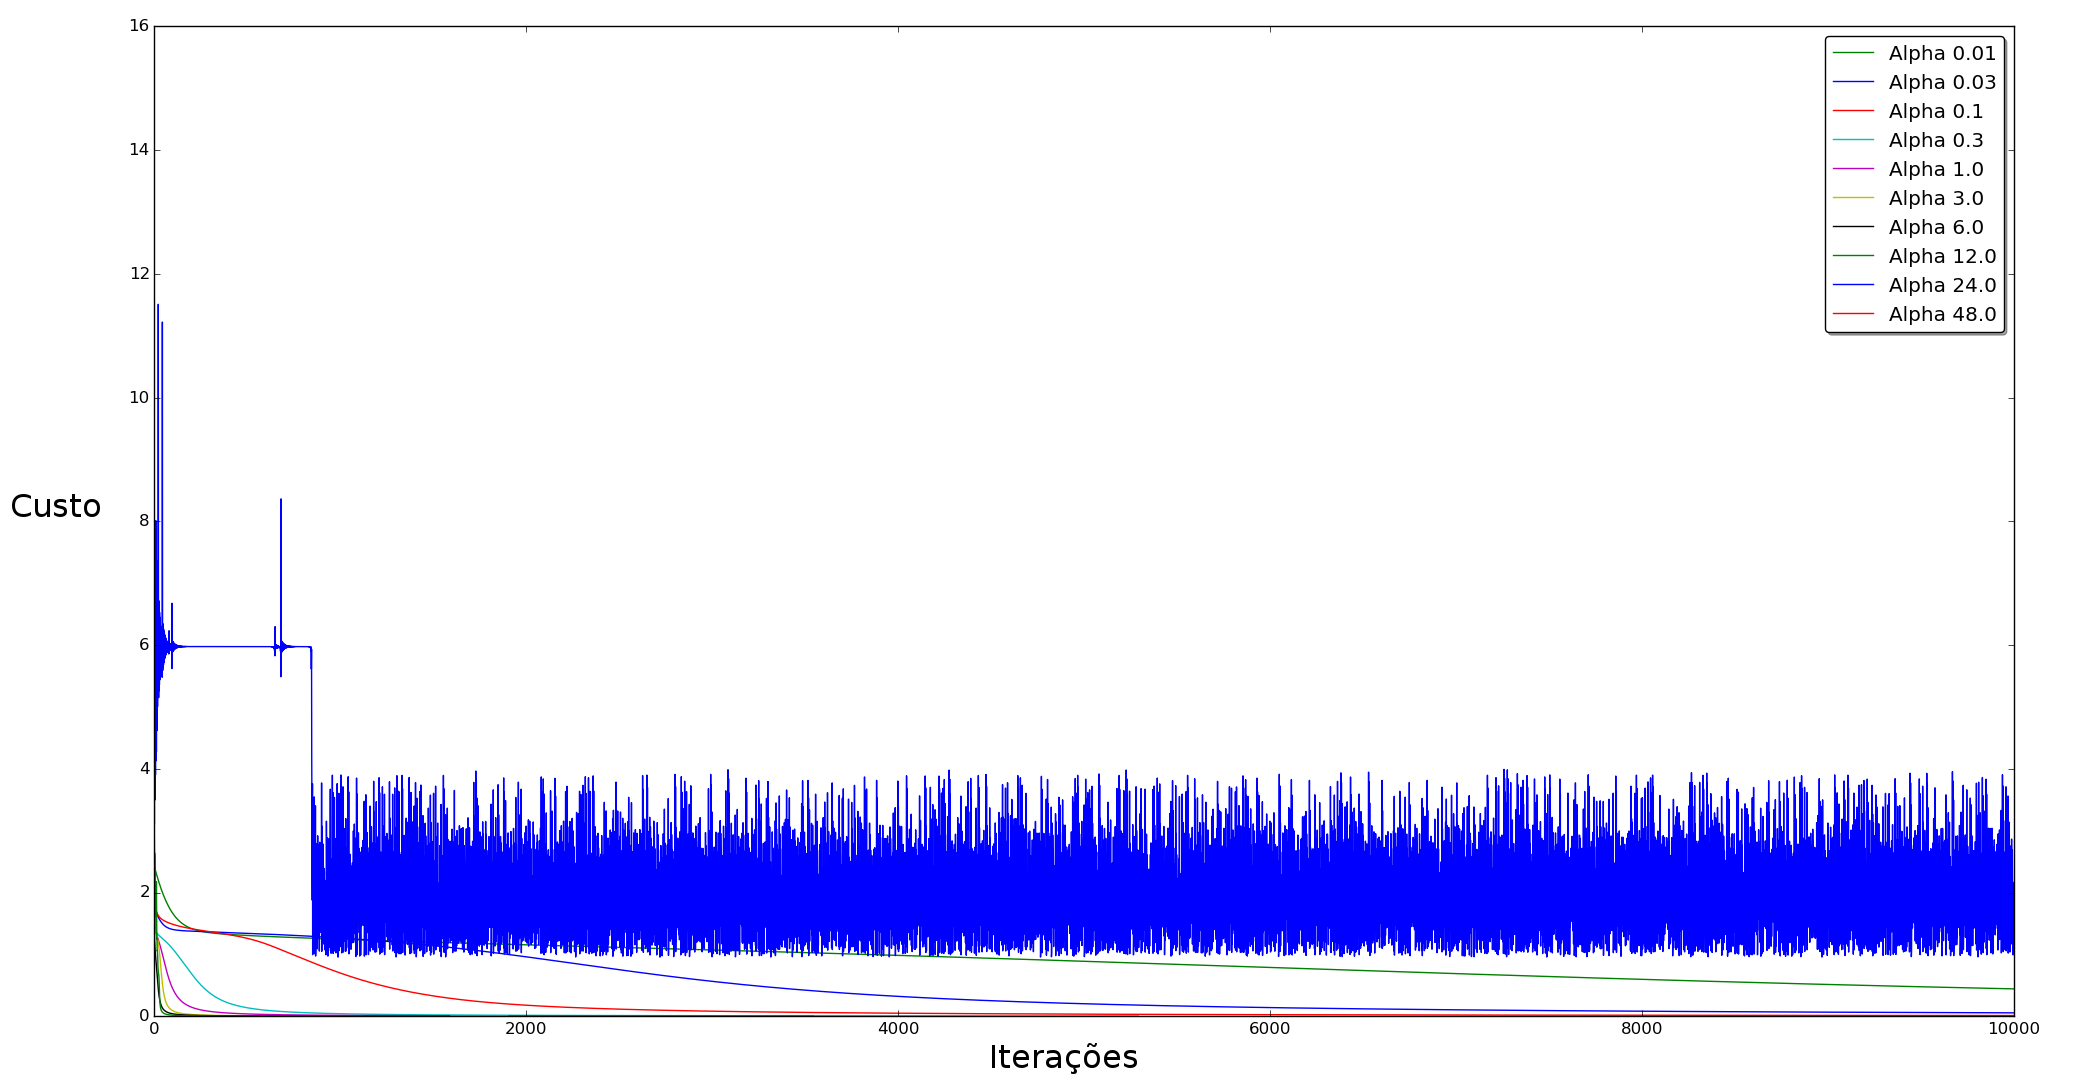
\includegraphics[scale=0.18]{img/alphas_rnn.png}
    \end{center}
    % \caption{Exemplo de classificação gramatical}\label{fig:exemploclassificacao}
  \end{figure}
  \end{adjustwidth}
\end{frame}



\begin{frame}
  \frametitle{Resultados - Redes Neurais}

  \begin{itemize}
  \item Com $\alpha$ igual a 3.0
 \end{itemize}

  \begin{adjustwidth}{-3em}{-3em}

    \begin{figure}[!htb]
    \begin{center}
    \begin{tikzpicture}[scale=1]
      \begin{axis}[
        name=one,
        mlineplot,
        width=1\textwidth,
        height=0.70\textwidth,
        xmode=normal,
        ymode=normal,
        ymin=0,
        ticks=both,
        xlabel=Unidades ocultas,
        ylabel=Tempo de execução (s),
        legend pos=north east,
        legend style={draw=none},
      ]
      \addplot table [x=grau,y=tempo,smooth,header=true,mark=none] {resultados_rnn/rnn_result_times_hidden.txt};
    \end{axis}

    \end{tikzpicture}
  \end{center}
  \end{figure}

  \end{adjustwidth}
\end{frame}



\begin{frame}
  \frametitle{Resultados - Redes Neurais}

  \begin{itemize}
  \item Com $\alpha$ igual a 3.0
 \end{itemize}

  \begin{adjustwidth}{-3em}{-3em}

    \begin{figure}[!htb]
    \begin{center}
    \begin{tikzpicture}[scale=1]
      \begin{axis}[
        name=one,
        mlineplot,
        width=1\textwidth,
        height=0.70\textwidth,
        xmode=normal,
        ymode=normal,
        ymin=0,
        ticks=both,
        xlabel=Unidades ocultas,
        ylabel=Número de iterações,
        legend pos=north east,
        legend style={draw=none},
      ]
      \addplot table [x=grau,y=iters,header=true,mark=none]  {resultados_rnn/rnn_result_iters_hidden.txt};
    \end{axis}

    \end{tikzpicture}
  \end{center}
  \end{figure}

  \end{adjustwidth}
\end{frame}


\begin{frame}
  \frametitle{Resultados - Redes Neurais}

  \begin{itemize}
  \item Com $\alpha$ igual a 3.0
 \end{itemize}

  \begin{adjustwidth}{-3em}{-3em}

    \begin{figure}[!htb]

    \begin{center}
    \begin{tikzpicture}[scale=1]
      \begin{axis}[
        name=one,
        mlineplot,
        width=1\textwidth,
        height=0.70\textwidth,
        xmode=normal,
        ymode=normal,
        ymin=0,
        ticks=both,
        xlabel=Unidades ocultas,
        ylabel=Acurácia (\%),
        legend pos=north east,
        legend style={draw=none},
      ]
      \addplot table [x=grau,y=acc,header=true,mark=none]  {resultados_rnn/rnn_result_accs_hidden.txt};
    \end{axis}

    \end{tikzpicture}
  \end{center}
  \end{figure}

  \end{adjustwidth}
\end{frame}








\begin{frame}
  \frametitle{Resultados - Redes Neurais}

  \begin{itemize}
  \item Com $\alpha$ igual a 3.0
 \end{itemize}

  \begin{adjustwidth}{-3em}{-3em}
  \begin{figure}[htb]
    \begin{center}
        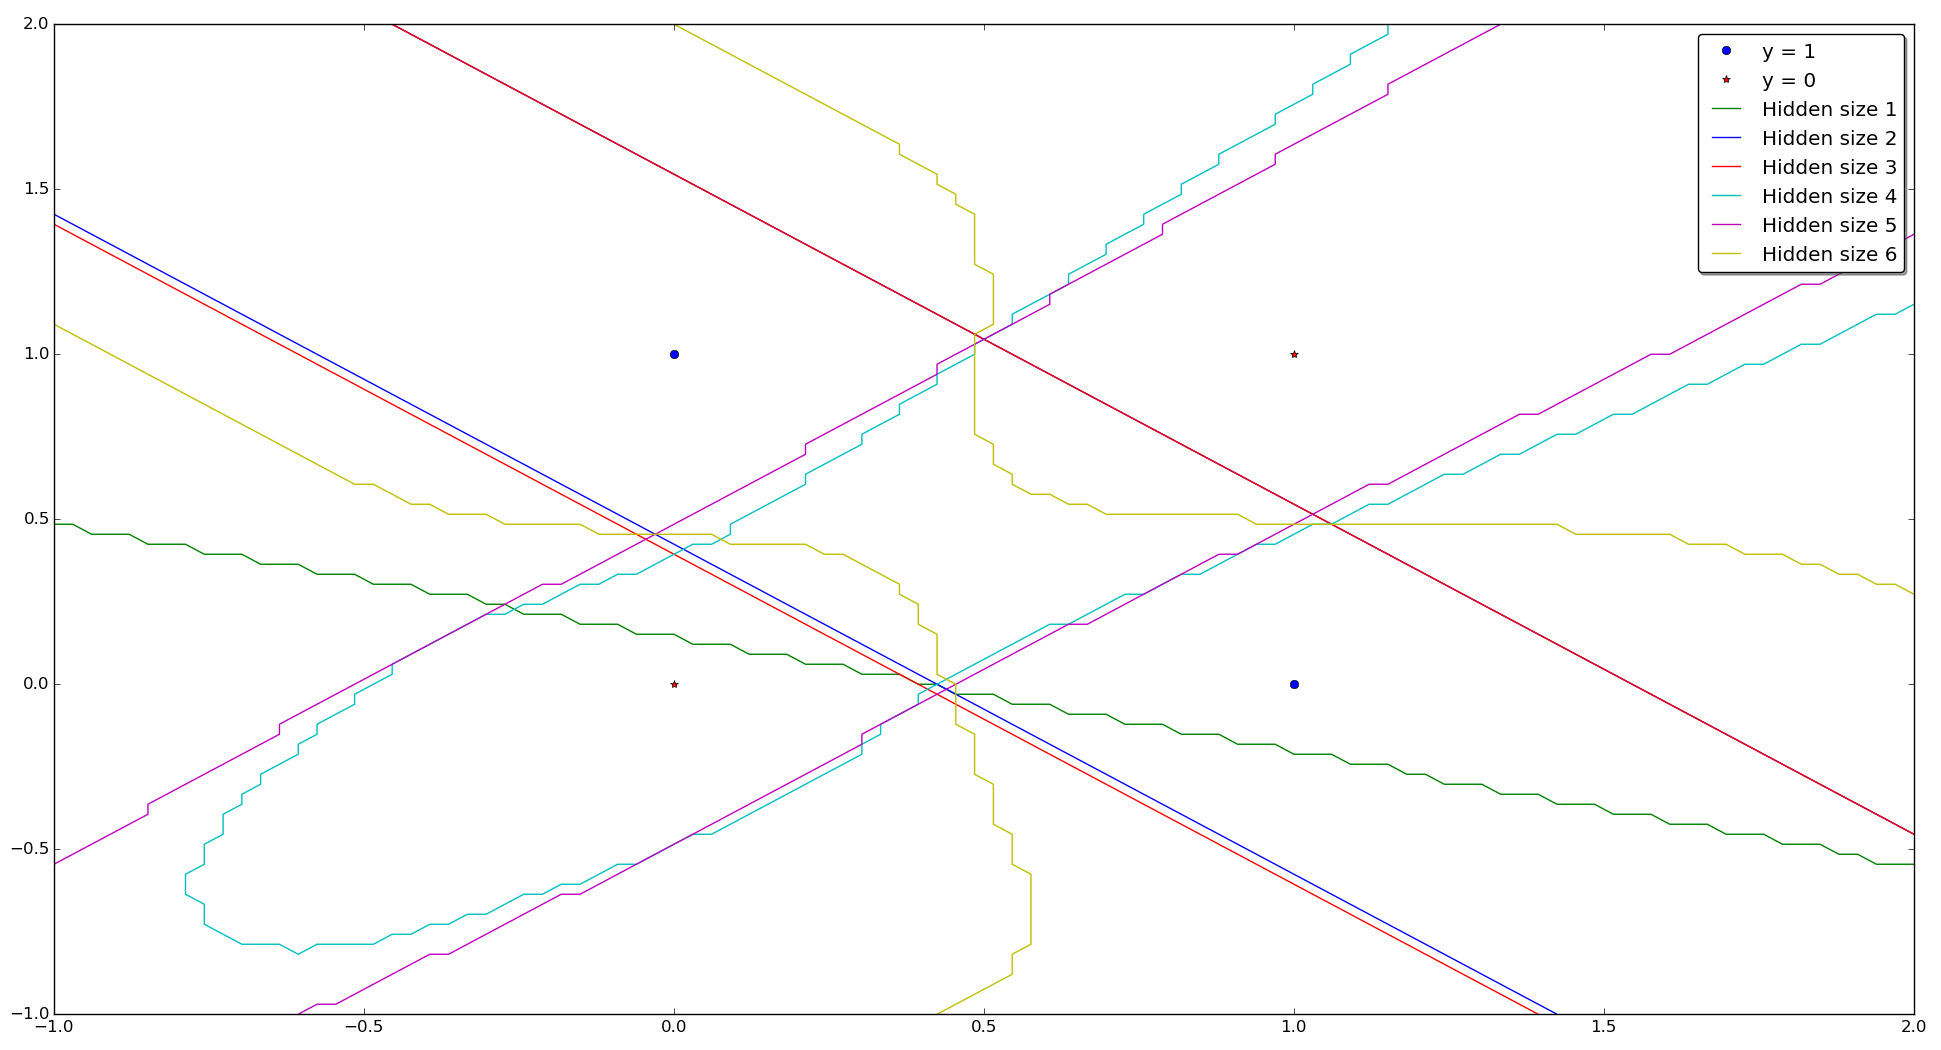
\includegraphics[scale=0.18]{img/boundaries_rnns_new.png}
    \end{center}
    % \caption{Exemplo de classificação gramatical}\label{fig:exemploclassificacao}
  \end{figure}
  \end{adjustwidth}
\end{frame}



\begin{frame}
  \frametitle{Resultados - Regressão Logística x Redes Neurais}


  \begin{itemize}
  \item Com grau do polinômio igual a 2 e 6 unidades ocultas
 \end{itemize}

  \begin{adjustwidth}{-3em}{-3em}

    \begin{figure}[!htb]

    \begin{center}
    \begin{tikzpicture}[scale=1]
      \begin{axis}[
        name=one,
        mlineplot,
        width=1\textwidth,
        height=0.70\textwidth,
        xmode=normal,
        ymode=normal,
        ymin=0,
        ticks=both,
        xlabel=Taxa de aprendizagem,
        ylabel=Tempo (s),
        legend pos=north east,
        legend style={draw=none},
      ]

      \addplot table [x=alpha,y=tempo,header=true,mark=none]  {resultados_rl/reg_result_times.txt};
       \addlegendentry{Regressão Logística}

      \addplot table [x=alpha,y=tempo,header=true,mark=none]  {resultados_rnn/rnn_result_times.txt};
       \addlegendentry{Redes Neurais}

      

      % \addplot+[BrickRed] table [x=tamanho,y=consulta4,header=true] {resultados1.txt};
   
    \end{axis}

    \end{tikzpicture}
  \end{center}
  \end{figure}

  \end{adjustwidth}
\end{frame}




\begin{frame}
  \frametitle{Resultados - Regressão Logística x Redes Neurais}

   \begin{itemize}
  \item Com grau do polinômio igual a 2 e 6 unidades ocultas
 \end{itemize}

  \begin{adjustwidth}{-3em}{-3em}

    \begin{figure}[!htb]

    \begin{center}
    \begin{tikzpicture}[scale=1]
      \begin{axis}[
        name=one,
        mlineplot,
        width=1\textwidth,
        height=0.70\textwidth,
        xmode=normal,
        ymode=normal,
        ymin=0,
        ticks=both,
        xlabel=Taxa de aprendizagem,
        ylabel=Iterações,
        legend pos=north east,
        legend style={draw=none},
      ]

      \addplot table [x=alpha,y=iters,header=true,mark=none]  {resultados_rl/reg_result_iters.txt};
       \addlegendentry{Regressão Logística}

      \addplot table [x=alpha,y=iters,header=true,mark=none]  {resultados_rnn/rnn_result_iters.txt};
       \addlegendentry{Redes Neurais}

      

      % \addplot+[BrickRed] table [x=tamanho,y=consulta4,header=true] {resultados1.txt};
   
    \end{axis}

    \end{tikzpicture}
  \end{center}
  \end{figure}

  \end{adjustwidth}
\end{frame}



\begin{frame}
  \frametitle{Resultados - Regressão Logística x Redes Neurais}
   \begin{itemize}
  \item Com grau do polinômio igual a 2 e 6 unidades ocultas
 \end{itemize}
  \begin{adjustwidth}{-3em}{-3em}

    \begin{figure}[!htb]

    \begin{center}
    \begin{tikzpicture}[scale=1]
      \begin{axis}[
        name=one,
        mlineplot,
        width=1\textwidth,
        height=0.70\textwidth,
        xmode=normal,
        ymode=normal,
        ymin=0,
        ticks=both,
        xlabel=Taxa de aprendizagem,
        ylabel=Acurácia (\%),
        legend pos=north east,
        legend style={draw=none},
      ]

      \addplot table [x=alpha,y=acc,header=true,mark=none]  {resultados_rl/reg_result_accs.txt};
       \addlegendentry{Regressão Logística}

      \addplot table [x=alpha,y=acc,header=true,mark=none]  {resultados_rnn/rnn_result_accs.txt};
       \addlegendentry{Redes Neurais}

      

      % \addplot+[BrickRed] table [x=tamanho,y=consulta4,header=true] {resultados1.txt};
   
    \end{axis}

    \end{tikzpicture}
  \end{center}
  \end{figure}

  \end{adjustwidth}
\end{frame}





\begin{frame}
  \frametitle{Resultados - Regressão Logística x Redes Neurais}
   \begin{itemize}
  \item Com grau do polinômio igual a 2 e 6 unidades ocultas
 \end{itemize}
  \begin{adjustwidth}{-3em}{-3em}

    \begin{figure}[!htb]

    \begin{center}
    \begin{tikzpicture}[scale=1]
      \begin{axis}[
        name=one,
        mlineplot,
        width=1\textwidth,
        height=0.70\textwidth,
        xmode=normal,
        ymode=normal,
        ymin=0,
        ticks=both,
        xlabel=Taxa de aprendizagem,
        ylabel=Custo - J(W),
        legend pos=north east,
        legend style={draw=none},
      ]

      \addplot table [x=alpha,y=custo,header=true,mark=none]  {resultados_rl/reg_result_alphas.txt};
       \addlegendentry{Regressão Logística}

      \addplot table [x=alpha,y=custo,header=true,mark=none]  {resultados_rnn/rnn_result_alphas.txt};
       \addlegendentry{Redes Neurais}

      

      % \addplot+[BrickRed] table [x=tamanho,y=consulta4,header=true] {resultados1.txt};
   
    \end{axis}

    \end{tikzpicture}
  \end{center}
  \end{figure}

  \end{adjustwidth}
\end{frame}




\section{Conclusão}

\begin{frame}[fragile]
  \frametitle{Conclusão}

  \begin{itemize}

    \item Regressão logística generaliza melhor que redes neurais

    \item Regressão logística é mais rápida para convergir para o problema do XOR

    \item Regressão logística tem o custo extra de calcular features polinomiais

    \item Regressão logística precisa de pelo menos um polinômio de grau 2 para classificar corretamente

    \item Redes neurais começa a divergir após um determinado valor de taxa de aprendizado

    \item Redes neurais teve boa acurácia com 3+ unidades ocultas

    \item É importante testar os hiper parâmetros!

  \end{itemize}

\end{frame}









\plain{Comparativo de Regressão Logística e Redes Neurais para classificação do XOR \\ \ \\ \normalsize{Marcos Treviso\\Sharbell Kemel} \\ \ \\ \ \\ {Aprendizado de Máquina} \\ \ \\ \ \\ {\normalsize 3 de outubro de 2015} \\ {\scriptsize Universidade Federal do Pampa}}




\end{document}
